\documentclass{article}
\usepackage{tikz}
\usetikzlibrary{arrows.meta,calc,positioning,shapes.geometric}
\begin{document}
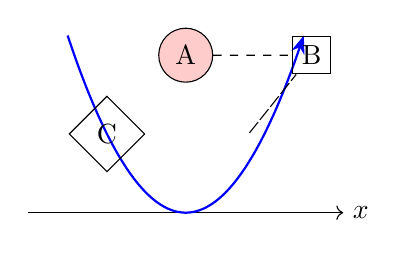
\begin{tikzpicture}
  \draw[->] (-2,0) -- (2,0) node[right] {$x$};
  \draw[-{Stealth}, thick, blue] plot[domain=-1.5:1.5, smooth] (\x, {\x*\x});
  \node[draw, circle, fill=red!20] (a) at (0,2) {A};
  \node[draw, rectangle, right=of a] (b) {B};
  \draw[dashed] (a) -- (b) -- ($(a)!0.5!(b) + (0,-1)$) -- cycle;
  \node[draw, diamond] at (-1,1) {C};
\end{tikzpicture}
\end{document}
